\documentclass{standalone}
\usepackage{tikz}
\usetikzlibrary{snakes}
\usetikzlibrary{shapes.geometric}
\usetikzlibrary{shapes.misc}

\begin{document}

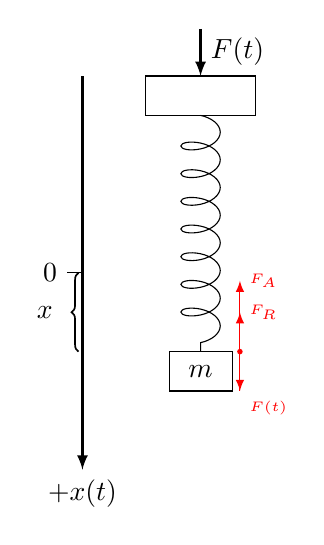
\begin{tikzpicture}[>=latex]
	\draw [->, thick] (0,3) -- (0,-2) node [below] {\(+x(t)\)};
	\draw (0,0.5) --++ (-0.2,0) node [left] {\(0\)};
	\draw [semithick ,snake = brace, mirror snake] (-0.05,0.5) to node [midway, left=2mm] {\(x\)} ++(0,-1);
	\draw (0.8,2.5) rectangle ++(1.4,0.5);
	\draw [snake = coil, segment amplitude = 0.25cm] (1.5,2.5) --++ (0,-3);
	% \draw (1.5,1) --++ (0,-0.3);
	\draw (1.1,-0.5) rectangle node {\(m\)} ++(0.8,-0.5);
	\draw [red,<->] (2,-1)  node [below right] {\tiny \(F(t)\)} --++ (0,1.4) node [above, right] {\tiny \(F_A\)};
	\draw [red,->] (2,-1) --++ (0,1) node [right] {\tiny \(F_R\)};
	\fill [red] (2,-0.5) circle (1pt);
	\draw [thick ,->] (1.5,3.6) --++ (0,-0.6) node [above right] {\(F(t)\)};
\end{tikzpicture}

\end{document}
